\nonstopmode

\title{Row-level MAC in H2}
\author{Christopher Martin\\{\tt chris.martin@gatech.edu}}

\documentclass[twocolumn]{article}

\usepackage{hyperref}\hypersetup{hidelinks}
\usepackage{graphicx}
\usepackage{verbatim}

\begin{document}

\twocolumn[
  \begin{@twocolumnfalse}
    \maketitle
    \begin{abstract}
      This project explores how a relational database manager can be modified to enforce a mandatory access control policy (MAC) using a multi-level security (MLS) model. As a prototype, I modified the H2 DBMS to enforce read permissions on a per-tuple granularity and include security-related additions to the SQL grammar.
      ~\\
    \end{abstract}
  \end{@twocolumnfalse}
]

\section{Motivation}

The aim is to help provide strong guarantees for information protection in information systems. In particular I consider the requirements of U.S. Department of Defense information systems, but the result is conceivably generalizable to other domains, notably for the protection of patient privacy in healthcare systems.

\begin{figure}
  \begin{center}
    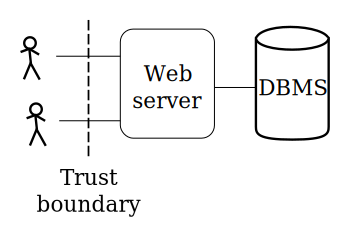
\includegraphics[width=0.5\linewidth]{webapp.pdf}
  \end{center}
  \caption{A common web architecture with a web application server and DBMS in the same trust domain.}
  \label{fig:webapp}
\end{figure}

As a typical example of an information system architecture, consider a mostly-stateless web application using a relational database for persistence, depicted in Figure \ref{fig:webapp}. In this picture, the web application connects to a database with permissions sufficient to access data for all users of the system.

\begin{figure}
  \begin{center}
    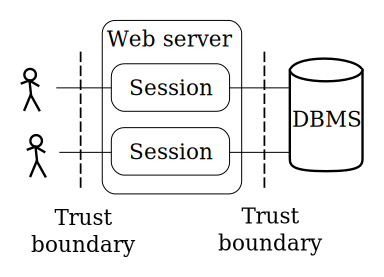
\includegraphics[width=0.5\linewidth]{webapp2.pdf}
  \end{center}
  \caption{Architecture one in which the DBMS has sufficient power to distrust its clients, enforcing an additional trust boundary.}
  \label{fig:webapp2}
\end{figure}

Instead we strive for the alternative of Figure \ref{fig:webapp2}. In this design, each user's session corresponds to a dedicated database connection associated with that user's credentials. Even if the server suffers from a SQL injection vulnerability that allows a user to execute arbitrary queries, since the database itself is responsible for enforcing access control, the user is unable to gain unauthorized access. The web server is still a trusted component of the system, but the complexity of its burden has been largely reduced to simply avoiding crosstalk between sessions.

Oracle has a similar extension to Oracle Database called Oracle Label Security (OLS)\cite{ols}.

\section{Security model}

Here we consider a slightly simplified variant of the multilevel security (MLS) model utilized in U.S. Department of Defense information systems.\cite{tcsec}

\begin{description}

  \item[Sensitivity level] A fully ordered set of labels. Herein we call these labels $0$, $1$, $2$, and $3$, where the infimum level $0$ denotes the least sensitive data, and the supremum level $3$ is applied to the most highly-guarded secrets.

  \item[Compartment] A set of labels indicating topics to which data pertains. This set is partially ordered because topics may be nested hierarchically. For example, if the compartment {\it Food} contains the compartments {\it Apples} and {\it Oranges}, then ${\it Food} > {\it Bananas}$, but {\it Apples} and {\it Oranges} are incomparable.

  \item[Marking] A marking consists of one sensitivity level and one or more compartments. We denote this by separating the components with slashes, such as {\it 2/Apples/Bananas}. {\it 0} is a special case for which no compartments are permitted, because that sensitivity represents no access control whatsoever. Markings form a lattice where the infinum is {\it 0} and the supremum is a marking with the highest sensitivity and every compartment.

  \item[Credential] A credential consists of a sensitivity level and a compartment. Each subject has a set of credentials.

\end{description}

A subject has read access to data marked by {\it $\ell$/$C_1$/$C_2$/\ldots/$C_n$} only if for all $i \in [1, n]$ the subject has a credential ($\ell'$, $C'$) such that $\ell' \ge \ell$ and $C' \ge C_i$.

\begin{figure}
  \begin{center}
    \includegraphics[width=0.75\linewidth]{lattice.pdf}
  \end{center}
  \caption{The lattice of markings formed using sensitivities $\{0,1,2\}$ and compartments $\{A,B\}$. Arrows point from more restrictive to less restrictive markings.}
  \label{fig:lattice}
\end{figure}

\section{Implementation}

\subsection{The {\tt MAC} schema}

\begin{figure*}
  \begin{center}
    \includegraphics[width=\linewidth]{mac-schema.pdf}
  \end{center}
  \caption{The tables of the underlying {\tt MAC} schema.}
  \label{fig:mac-schema}
\end{figure*}

When a new database is initialized, it creates a schema called {\tt MAC} whose tables are given by Figure \ref{fig:mac-schema}. This stores sensitivities, compartments, markings, and users' credentials. The most critical use of these tables is to generate a table view in the {\tt MAC} schema called {\tt session\_marking}, a single-column relation containing an entry corresponding to each marking that the current session is permitted to access.

\subsection{SQL grammar modifications}

\begin{itemize}

\item When creating a new schema, the keyword {\tt restricted} enables the security feature.

{\tt create restricted schema "schema\_name";}

\item The {\tt grant} syntax is modified to allow granting MLS credentials to users.

{\tt grant marking $'$3/B$'$ to alice;}

\item The {\tt insert} syntax is modified to allow specification of a marking,

{\tt insert into people marked $'$2/B/C$'$ (name) values ($'$Bob$'$);}

\end{itemize}

\subsection{Query interpretation}

When a user creates a restricted schema,

\begin{quote}
{\tt create restricted schema vault;}
\end{quote}

the database actually creates two schemas.

\begin{quote}
{\tt create schema vault;\\
create schema vault\_shadow;}
\end{quote}

The ``shadow'' schema contains all of the relations created explicitly by {\tt create table} statements, and the other schema contains restricted views into those tables.

When we create a table called {\tt doc} on the {\tt vault} schema,

\begin{quote}
{\tt create table vault.doc (title varchar(20))}
\end{quote}

the database actually adds the table to the shadow schema, and places a restricted view into the visible schema.

\begin{quote}\begin{verbatim}
create table vault_shadow.doc (
  title varchar(20),
  marking_id bigint
);

create view vault.doc as
  select title,
  render_marking(marking_id)
  from vault_shadow.doc
  join mac.session_marking;
\end{verbatim}\end{quote}

Finally, when the database executes an {\tt insert} query,

\begin{quote}
{\tt insert into vault.doc marked $'$2/A$'$ (title) values ($'$hi$'$);}
\end{quote}

the database translates this into an insertion into the shadow table, with the marking string parsed and converted to a marking identifier.

\begin{quote}
{\tt insert into vault\_shadow.doc marked (title, marking\_id) values ($'$hi$'$, \ldots);}
\end{quote}

\section{Performance evaluation}

\begin{figure}
  \begin{center}
    \includegraphics[width=\linewidth]{test-schema.pdf}
  \end{center}
  \caption{The tables in the schemata used for testing.}
  \label{fig:test-schema}
\end{figure}

The test setup models a system for storing multi-page documents. The {\tt Document} and {\tt Page} tables are both separately protected with markings, so a user who can see a document may not be able to see all of its pages.

Figure \ref{fig:performance} shows how query execution time varies as a function of the size of the {\tt Document} relation. Using an on-disk database, the access control incurs a cost of roughly 37 milliseconds per document. H2 can also run purely in memory, in which can the penalty is only 3 milliseconds.

\begin{figure}
  \begin{center}
    \includegraphics[width=\linewidth]{performance.png}
  \end{center}
  \caption{Execution time for a query which joins all three tables.}
  \label{fig:performance}
\end{figure}

\end{description}

\bibliographystyle{plainnat}
\begin{thebibliography}{99}
\bibitem{tcsec}{Department of Defense. 1985. {\it Trusted Computer System Evaluation Criteria} (Orange Book). ``Division B: Mandatory protection''}
\bibitem{h2}{H2 database. \url{http://h2database.com/}}
\bibitem{ols}{Oracle Label Security. \url{http://www.oracle.com/us/products/database/options/label-security/overview/index.html}}
\end{thebibliography}

\end{document}
